\documentclass[12pt]{article}
\usepackage{geometry}                % See geometry.pdf to learn the layout options. There are lots.
\geometry{letterpaper}                   % ... or a4paper or a5paper or ... 
%\geometry{landscape}                % Activate for for rotated page geometry
\usepackage[parfill]{parskip}    % Activate to begin paragraphs with an empty line rather than an indent
\usepackage{daves,fancyhdr,natbib,graphicx,dcolumn,amsmath,lastpage,url}
\usepackage{amsmath,amssymb,epstopdf,longtable}
\usepackage{paralist}  % need to properly formulate standard answer blocks
\usepackage[final]{pdfpages}
\DeclareGraphicsRule{.tif}{png}{.png}{`convert #1 `dirname #1`/`basename #1 .tif`.png}
\pagestyle{fancy}
\lhead{CE 3305 Fluid Mechanics; Final Exam Part 2 (In Class)}
\rhead{Name:\_\_\_\_\_\_\_\_\_\_\_\_\_\_\_\_\_\_\_\_\_\_\_\_\_\_\_\_\_\_\_\_\_\_}
\lfoot{REVISION A}
\cfoot{}
\rfoot{Page \thepage\ of \pageref{LastPage}}
\renewcommand\headrulewidth{0pt}
%%%%%%%%%%%%%%%%%%%%%%%%%%%%%%%%%%%%
\begin{document}
%%%%%%%%%%%%%%%%%%%%%%%%%%%%%%%%%%%
\begingroup
\begin{center}
{\textbf{{ CE 3305 Engineering Fluid Mechanics} \\ Final Exam (Part 2) \\ Summer 2019 -- GERMANY} }
\end{center}
\endgroup
\begingroup
~\newline

\begin{enumerate}
%\item (Problem 9.42 pg 355) A flat plate 1.5 $m$ long and 1.0 $m$ wide is towed in water at 20$^oC$ in the direction of its length and at a speed of 15 $cm/s$.  Determine the resistance of the plate and the boundary layer thickness at its aft end.
%
%\item (Problem 9.48 pg 355) An airplane wing of 2$m$ chord length (leading edge to trailing edge distance)and 11 $m$ span flies at 200 $km/hr$ in air at 30$^oC$.  Assume the resistance of the wing surfaces is like that of a flat plate.
%\begin{enumerate}
%\item What is the friction drag on the wing?
%\item What power will be required to overcome this friction?
%\item How much of the chord is laminar?
%\item What will be the change in drag if a turbulent boundary layer is tripped at the leading edge?
%\end{enumerate}


\item Figure \ref{fig:WindDrum} is a schematic of wind blowing on a petroleum storage drum.  Estimate the wind speed (in meters per second) needed to tip the drum over.  \\~\\ The mass of the drum is 25 kilograms, the diameter is 55 centimeters, and the height is 90 centimeters.  \\~\\The density of air is $\rho = 1.23~kg/m^3$  \\ The viscosity of air is $\nu = 1.46 \times 10^{-5}~m^2/s$
\begin{figure}[htbp] %  figure placement: here, top, bottom, or page
   \centering
   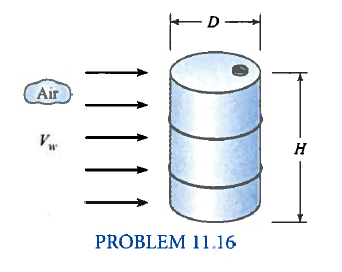
\includegraphics[width=2in]{WindDrum.jpg} 
   \caption{Wind blowing over a storage drum}
   \label{fig:WindDrum}
\end{figure}
\end{enumerate}
\clearpage
\textbf{Solution}\\
The problem statement is on the prior page, the first step is to sketch the situation and construct a free-body/flow diagram.\\
\textbf{Sketch}\\
\begin{figure}[h!] %  figure placement: here, top, bottom, or page
   \centering
   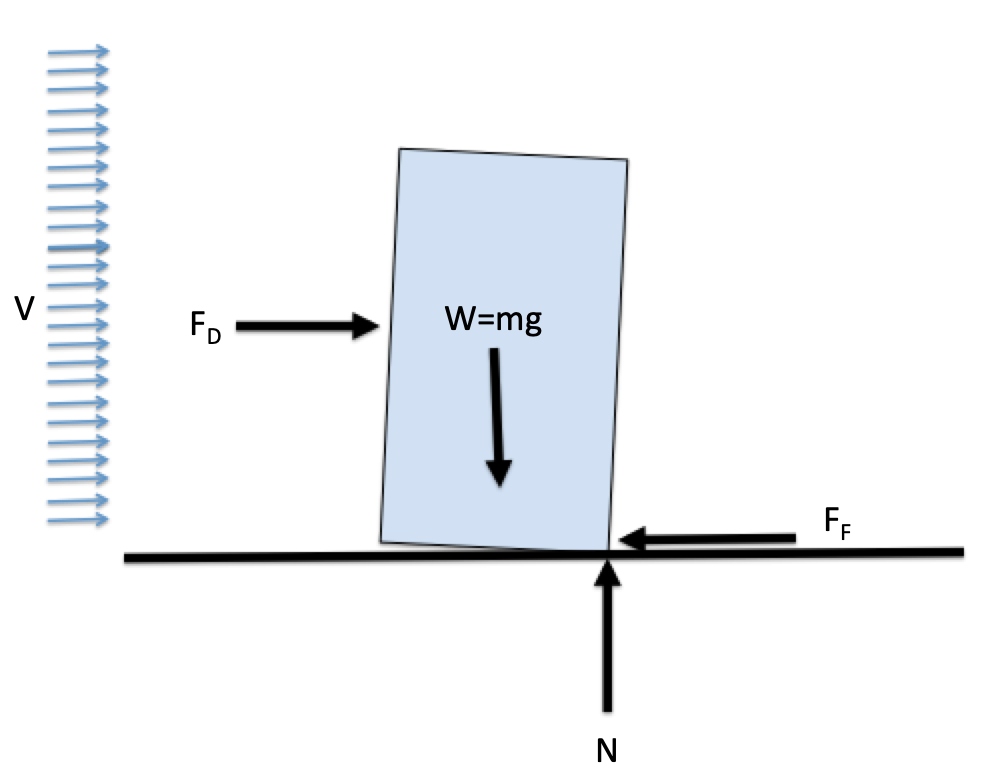
\includegraphics[width=4in]{Sketch.png} 
   \caption{Wind blowing over a storage drum}
   \label{fig:Sketch}
\end{figure}

\textbf{Given}\\
Next list the given information -- in this case we have the dimensions and the fluid properties.  Also given is the Fig 11.5 of the textbook which will be important.\\
The variables we will use are:
\begin{itemize}
\item H = 0.9 meters
\item D = 0.55 meters
\item m = 25 kg
\item  $\rho = 1.23~kg/m^3$
\item $\nu = 1.46 \times 10^{-5}~m^2/s$
\end{itemize}

\textbf{Find}\\
The velocity, $V$, in meters per second.\\
\textbf{Governing Equations}\\
The governing principles used are a static balance of forces on the drum:
\begin{equation}
\sum F = ma = 0 
\end{equation}
Also, at the moment the drum begins to tip over, the moment about the tip axis (A) is zero (overturning moment and righting moment are the same).
\begin{equation}
\sum M = 0 
\end{equation}
The drag force equation that will relate drag coefficient and velocity is
\begin{equation}
F_D = C_D\times A \times \frac{\rho V^2}{2}
\end{equation}
The Reynolds number for flow, based on cylinder diameter is
\begin{equation}
Re_D = \frac{V \times D}{\nu}
\end{equation}
\textbf{Analysis}
Using the momentum balance we have:
\begin{equation}
\frac{F_D H}{2} - \frac{mg D}{2} = 0
\end{equation}
After cancellation of common terms,
\begin{equation}
{F_D H}=mg D
\end{equation}
Now substitute the drag force formula for $F_D$.
\begin{equation}
{ C_D\times A \times \frac{\rho V^2}{2} H}=mg D
\end{equation}
Algebra to rearrange the equation
\begin{equation}
V=\sqrt{ \frac{2 mg D}{\rho \times C_D\times A \times H} }
\end{equation}
Next use the definition of projected area, $A=D \times H$ and substitute
\begin{equation}
V=\sqrt{ \frac{2 mg D}{\rho \times C_D\times D \times H \times H} }
\end{equation}
Cancel the diameters
\begin{equation}
V=\sqrt{ \frac{2 mg }{\rho \times C_D \times H^2} }
\end{equation}
Now build a computation table.
The first column is a guess of the velocity.
Then the Reynolds number is computed and used to look up the drag coefficient, $C_D$.
Next the value is used in the velocity equation to compute velocity based on the analysis.
The guess is adjusted until the two values are equal (or less than some difference tolerance)

% Requires the booktabs if the memoir class is not being used
\begin{table}[h!]
   \centering
   %\topcaption{Table captions are better up top} % requires the topcapt package

      \caption{Table of Velocity Guess and Check}
     \begin{tabular}{p{1in}p{1in}p{1in}p{1in}p{1in}}
     $V_{guess}$ (m/s) & $Re_D$ & $C_D$ & $V_{comp}$ (m/s) & Rel.Error\\ 
     \hline
     \hline
     10&376712&0.19&47.45&-78\%\\
      20&753424&0.21&45.5&-56\%\\
      30&1130136&0.31&37.70&-20.4\%\\
      35& 1318493&0.34&35.86&-2.3\%\\
      35.6& 1341095&0.348& 35.66&-0.1\%\\
     \hline
   \end{tabular}

   \label{tab:booktabs}
\end{table}

\begin{figure}[h!] %  figure placement: here, top, bottom, or page
   \centering
   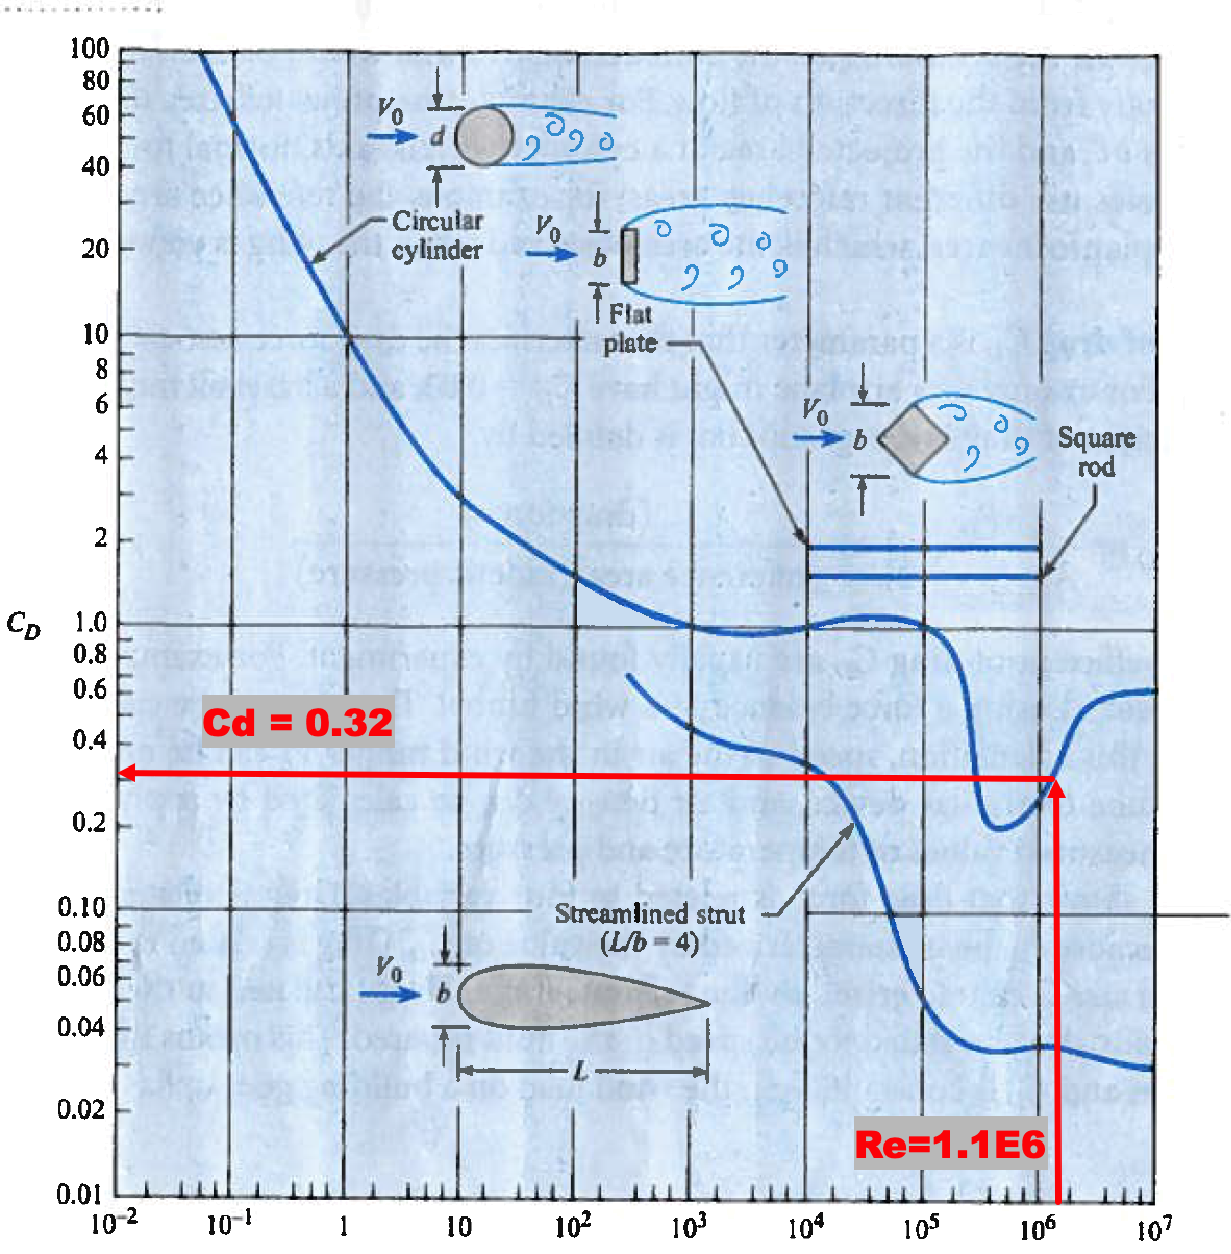
\includegraphics[width=5in]{Fig11-5.pdf} 
   \caption{Figure 11.5 from Fluid Mechanics Textbook}
   \label{fig:Fig11.5}
\end{figure}

Lastly we should check our work.

First, verify the Reynolds number:

\begin{equation}
Re_D = \frac{V \times D}{\nu} =  \frac{35.6 \times 0.55}{1.46 \times 10^{-5}} = 1.34 \times 10^{6}
\end{equation}

Next look up the drag coefficient, $C_D = 0.348$ (close to the value in the chart).

A tool to return the drag coefficient based on the Reynolds number is located at\\
\url{http://theodore-odroid.ttu.edu/documents/toolbox/fluidmechanics/DragOnCylinder/DragOnCylinder.html}\\
\begin{figure}[h!] %  figure placement: here, top, bottom, or page
   \centering
   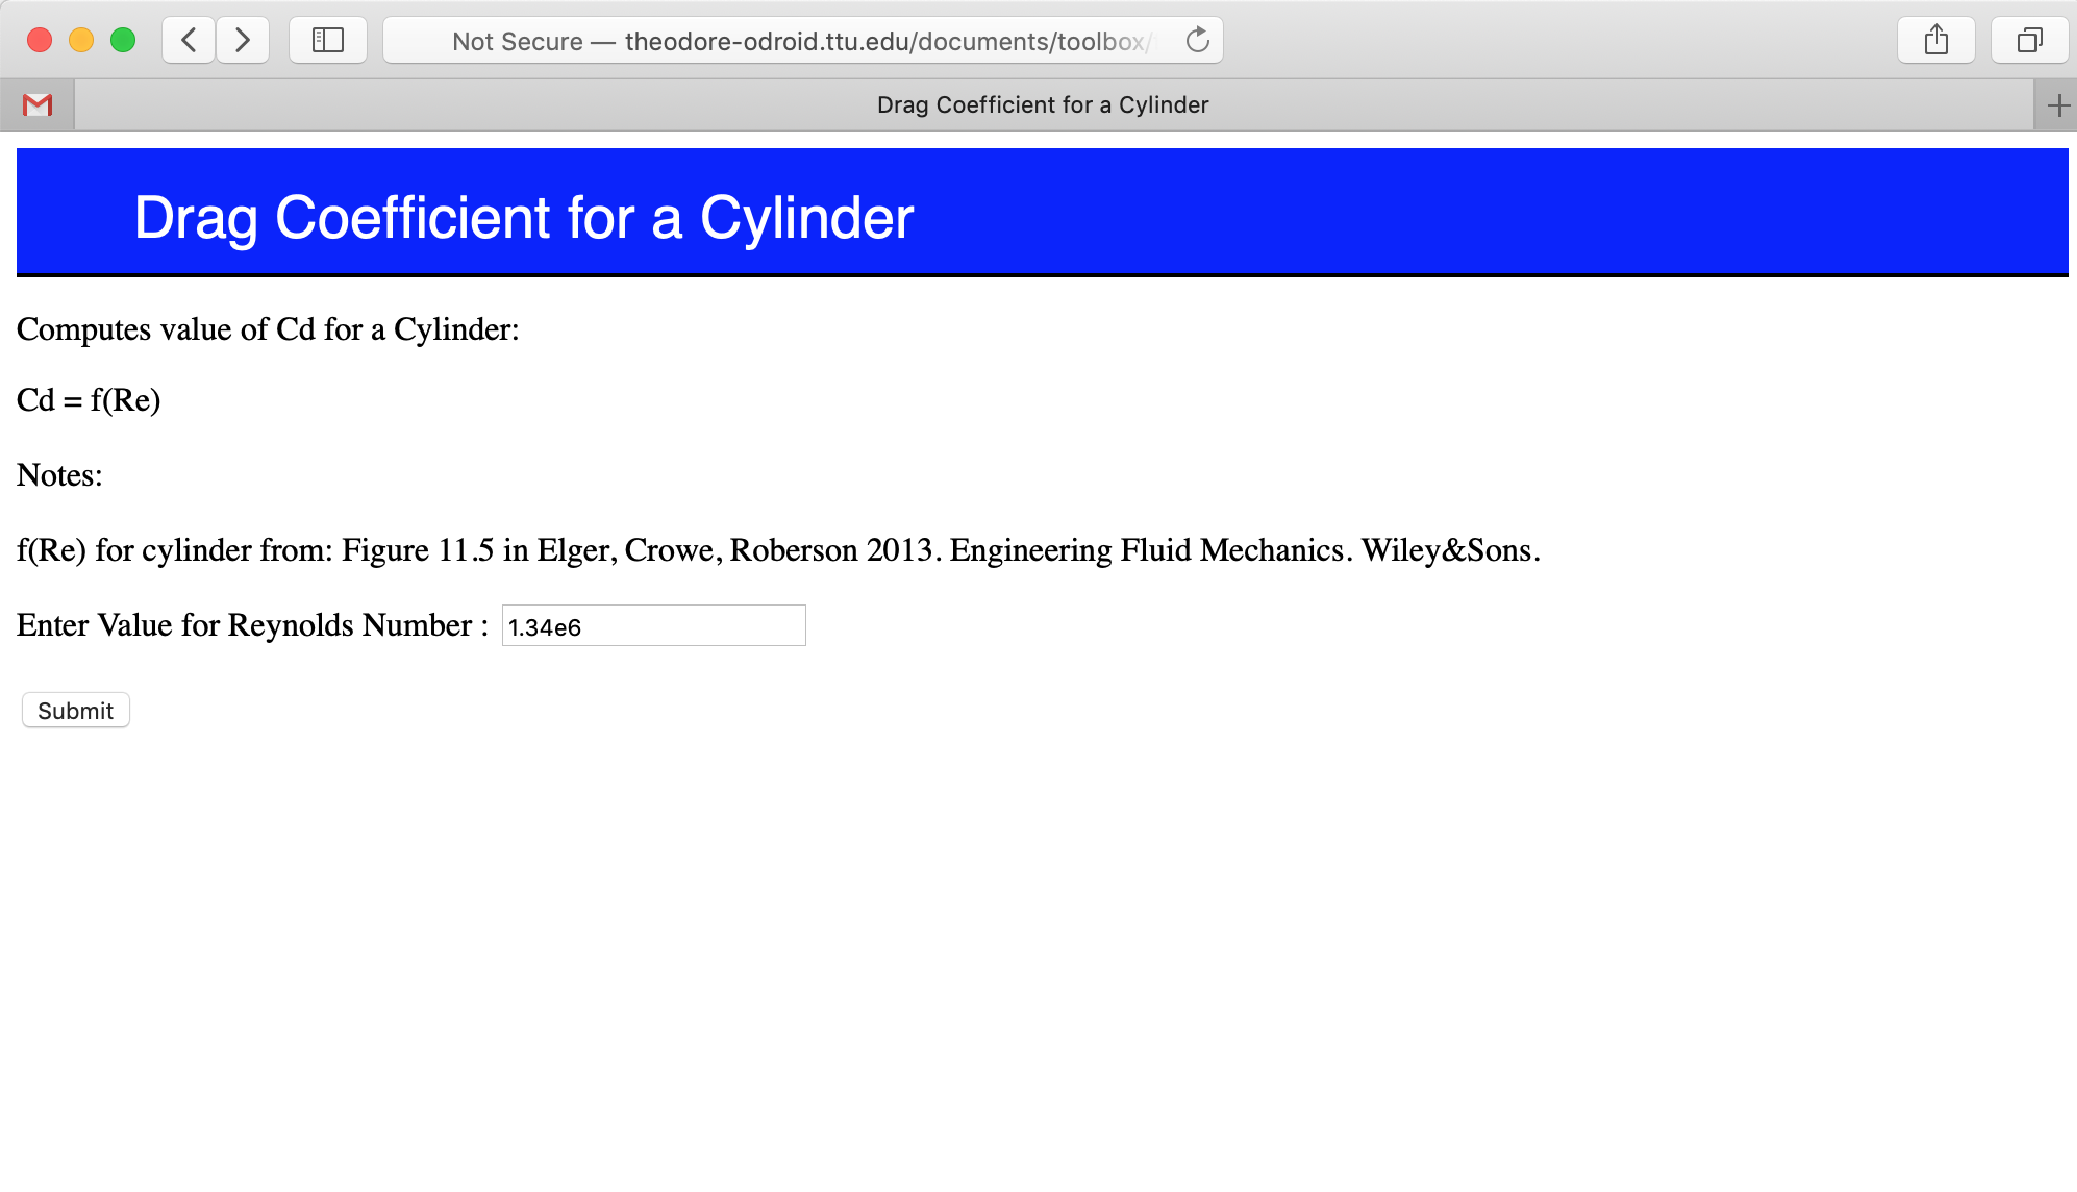
\includegraphics[width=6in]{CdInterface.pdf} 
   \caption{Drag coefficient web interface for Cd on a Cylinder}
   \label{fig:CdInterface}
\end{figure}
\newline
Figure \ref{fig:CdComputed} is the tool applied to the Reynolds number of $1.34 \times 10^{6}$
\begin{figure}[h!] %  figure placement: here, top, bottom, or page
   \centering
   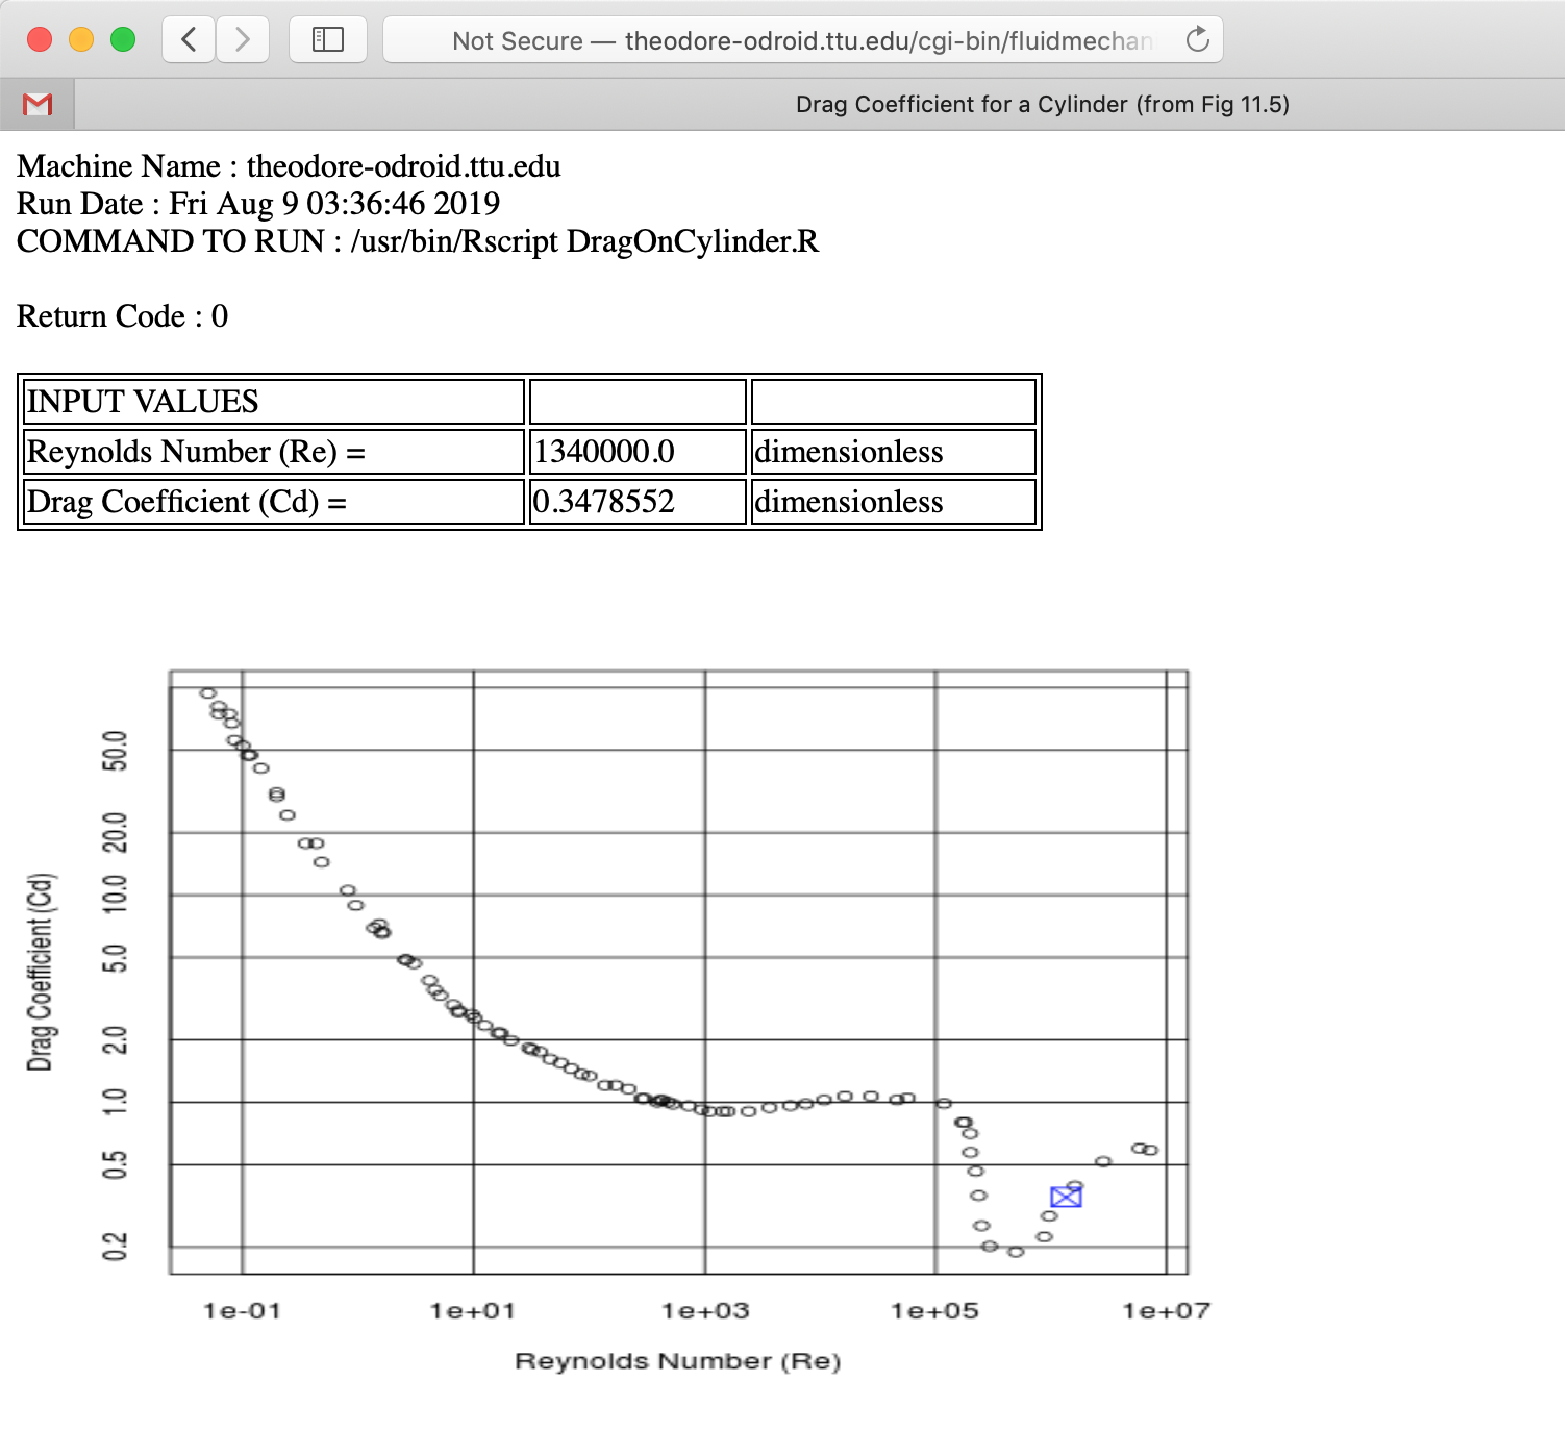
\includegraphics[width=5in]{CdComputed.pdf} 
   \caption{Drag Coefficient for Cylinder with Reynolds number of 1.34 million.}
   \label{fig:CdComputed}
\end{figure}

Next apply the velocity equation

\begin{equation}
V=\sqrt{ \frac{(2)(25)(9.8) }{(1.23)(0.348)(0.9)^2} } = 37.53 m/s
\end{equation}

So the values used are fairly close.

Thus the result in the table makes sense, hence report the velocity to tip the barrel as $35.6 m.s$ (about 70 miles per hour, which is a high wind speed but not unheard of!)
\clearpage

A listing to automate the calculations (which was used to build the table is)
\begin{verbatim}
# Script to return Drag Coefficient for a Cylinder Given Reynolds Number
# Uses digitized file from figure 11.5 in Fluid Mechanics Textbook
# Read the data file
zztop <- read.table("Cd-vs-Re-Cylinder.dat")
# Order the data
newdata <- zztop[order(zztop$V1),]  #V1 is reynolds number, V2 is CD
# Prompt User for Reynolds number
#reynolds <- readline(prompt="Enter Reynolds Number: ")
#reynolds <- as.numeric(reynolds) #convert to numeric
# Interoplate in the data table
#dragCoef <- approx(newdata,xout = reynolds,rule=2)
#message("Drag Coefficient : ",dragCoef$y)
#
# Computations for Determining velocity on barrel to tip it over
mass <- as.numeric(readline(prompt="Enter Cylinder Mass (kg)         : "))
diameter <- as.numeric(readline(prompt="Enter Diameter (meters)      : "))
height <- as.numeric(readline(prompt="Enter Height (meters)          : "))
density <- as.numeric(readline(prompt="Enter Air Density (kg/m^3)    : "))
viscosity <- as.numeric(readline(prompt="Enter Air Viscosity (m^2/s) : "))
#
continue = "yes"
while(continue == "yes"){
velocity_guess <- as.numeric(readline(prompt="Guess Air Velocoity    : "))
reynolds <- diameter*velocity_guess/viscosity
dragCoef <- approx(newdata,xout = reynolds,rule=2)
message("Drag Coefficient : ",dragCoef$y)
velocity_target <- sqrt(2*mass*9.8/(dragCoef$y*density*height))
message("Guess Velocity   : ",velocity_guess)
message("Reynolds Number  : ",reynolds)
message("Drag Coefficient : ",dragCoef$y)
message("Target Velocity  : ",velocity_target)
continue <- readline(prompt="Continue (yes/no) : ")
}
\end{verbatim}
The input file that contains points digitized from Figure 11.5 is
\begin{verbatim}
0.0500483357985  94.0842677875
0.0803246374783  67.3906052182
0.143432463613  40.8475532134
0.243244807137  24.2459868579
0.482067348163  14.3940126551
0.954695709589  8.90972244666
1.6133428483  6.51687505979
2.58749141209  4.8670075784
3.02589477  4.66863518479
4.1454419615  3.8698583667
4.60733788629  3.48650132163
7.38145514819  2.77218929551
16.1556110172  2.15934573487
30.215028115  1.8282427009
31.8370230107  1.79054994777
37.2180755192  1.75381789333
45.8766510479  1.61359620874
56.5096499919  1.54790931319
69.6316954214  1.45420629913
85.8007969959  1.36617561662
100.302736884  1.33814934615
137.219563348  1.20584164495
168.904048208  1.2060941398
299.799030934  1.04265415991
388.970926371  1.00026174815
409.562047421  1.02142511749
431.395600575  1.02147858312
478.785695685  1.000471196
531.381734274  0.979895839786
725.932269938  0.959944593104
941.852769306  0.920915001107
1101.04350788  0.902022984157
1427.52759626  0.902259087008
1583.78609379  0.902353545451
2399.63162364  0.902731478123
3633.17020128  0.941630949063
5502.75722361  0.961906195202
7512.12747251  0.982515148453
10798.1189994  1.02479892371
16348.927807  1.06895838521
27482.0635911  1.06951805421
56883.5735842  1.04818087308
117823.32883  0.985244594142
179148.741673  0.799879408276
199180.321119  0.705747161591
199885.297275  0.57272710712
222549.839513  0.464827487031
235493.020825  0.354325747456
249453.224805  0.253689914347
292647.626609  0.201650757043
492453.691213  0.189503291715
869468.654696  0.224092815598
960899.745198  0.281997292914
1606138.7748  0.394089172917
2830768.72289  0.517316557898
5842710.69683  0.599191454234
7194354.77752  0.586930122954
0.116238323303  47.2678773001
0.196917870112  29.8710396378
0.432973465203  17.7352705203
0.81464690869  10.5282720807
1.61277293274  6.6544096836
1.5289857954  7.23381442756
1.37910814166  6.93715852233
2.58749141209  4.8670075784
9.57698708368  2.65947714741
10.0946622446  2.55081354657
12.4431285278  2.34687026721
17.0168587674  2.15945876399
20.9757350618  1.98680517959
0.0761246934307  74.8044312399
0.0618445638421  74.7887709916
0.0617572234299  81.3049443831
0.110355334215  47.2654032327
0.0992919652135  52.4624542722
0.0848761673763  55.8458399797
0.35175255103  17.7315576555
0.196778771673  31.1451637392
7.3840635787  2.71489315205
6.64614245355  2.95112658397
5.1170823072  3.27510236095
284.625769851  1.04259958592
219.142683332  1.15705655729
46229.1904988  1.02630196798
170081.765634  0.799837541459
\end{verbatim}



\end{document}  